% Fig. 4C replication report.
% The prose is the author's notebook text, transcribed verbatim. Two kinds of editorial mark:
%   \fillin{} (red)  -- a placeholder in the notebook, filled in
%   \fix{}    (blue) -- a factual correction, always with a footnote giving the original wording
% Every number comes from report/parameters.tex, generated from report/values.json.
\documentclass[11pt,a4paper]{article}

\usepackage[margin=2.5cm]{geometry}
\usepackage[T1]{fontenc}
\usepackage{lmodern}
\usepackage{amsmath}
\usepackage{graphicx}
\usepackage{booktabs}
\usepackage{ragged2e}
\usepackage{xcolor}
\usepackage[hidelinks]{hyperref}
\usepackage{enumitem}
\usepackage{caption}

\captionsetup{font=small,labelfont=bf,justification=raggedright,singlelinecheck=false}
\setlength{\parindent}{0pt}
\setlength{\parskip}{0.6em}
\RaggedRight                      % left-justified, ragged right edge

\definecolor{fillred}{HTML}{C0392B}
\definecolor{fixblue}{HTML}{1F5FA9}
\definecolor{rulegrey}{HTML}{999999}
\definecolor{boxgrey}{HTML}{F4F4F4}

\newcommand{\fillin}[1]{\textcolor{fillred}{#1}}
\newcommand{\fix}[1]{\textcolor{fixblue}{#1}}

% ---------------------------------------------------------------- code references
% Set \repourl to the repository base (e.g. https://github.com/OWNER/habermas-fig4c) and every
% code reference below becomes a permalink pinned to \repocommitfull. Left empty, they render as
% plain file:line references. This VM cannot create the remote: the exe.dev GitHub proxy serves
% only /repos/OWNER/REPO, so `gh repo create` returns 403.
\newcommand{\repourl}{}
% #1 raw path (for the URL), #2 escaped path (for display), #3 start, #4 end, #5 label
\newcommand{\CodeRef}[5]{%
  \ifx\repourl\empty
    \texttt{\small #2:#3--#4} {\small #5}%
  \else
    \href{\repourl/blob/\repocommitfull/#1\#L#3-L#4}{\texttt{\small #2:#3--#4} {\small #5}}%
  \fi}
\newcommand{\codebox}[1]{%
  \par\vspace{0.2em}%
  \noindent\colorbox{boxgrey}{\parbox{\dimexpr\linewidth-2\fboxsep}{%
    \sloppy\small\textbf{Code:}\; #1}}\par\vspace{0.3em}}

% GENERATED by report/build_parameters.py from report/values.json -- do not edit.
% Every number in the report comes from here.

\newcommand{\paperShare}{0.285}
\newcommand{\paperOpinions}{0.28}
\newcommand{\paperInitCand}{0.28}
\newcommand{\paperInitWin}{0.29}
\newcommand{\paperRevCand}{0.33}
\newcommand{\paperRevWin}{0.36}
\newcommand{\paperRevWinSE}{0.03}
\newcommand{\paperNRounds}{1047}
\newcommand{\paperFigAr}{0.64}
\newcommand{\paperFigBwithin}{0.96}
\newcommand{\paperMarginalRsq}{0.41}
\newcommand{\paperConditionalRsq}{0.45}
\newcommand{\paperFigArSq}{0.41}
\newcommand{\groupMin}{4}
\newcommand{\groupMax}{5}
\newcommand{\groupNRounds}{1047}
\newcommand{\shareRuleNeutralDropped}{0.289}
\newcommand{\shareRuleNeutralDroppedNRounds}{560}
\newcommand{\shareRuleTiesKept}{0.284}
\newcommand{\shareRuleTiesKeptNRounds}{659}
\newcommand{\oursShareBase}{0.262}
\newcommand{\oursOpinionsBase}{0.263}
\newcommand{\oursNRoundsBase}{560}
\newcommand{\oursNRoundsTotalBase}{1047}
\newcommand{\oursFigArBase}{0.56}
\newcommand{\oursFigBwithinBase}{0.86}
\newcommand{\oursInitCandBase}{0.211}
\newcommand{\oursInitCandSEBase}{0.015}
\newcommand{\oursInitCandBootSEBase}{0.018}
\newcommand{\oursInitWinBase}{0.160}
\newcommand{\oursInitWinSEBase}{0.019}
\newcommand{\oursInitWinBootSEBase}{0.020}
\newcommand{\oursRevCandBase}{0.209}
\newcommand{\oursRevCandSEBase}{0.010}
\newcommand{\oursRevCandBootSEBase}{0.017}
\newcommand{\oursRevWinBase}{0.199}
\newcommand{\oursRevWinSEBase}{0.018}
\newcommand{\oursRevWinBootSEBase}{0.018}
\newcommand{\oursMarginalRsqGapBase}{0.119}
\newcommand{\oursMarginalRsqBase}{0.291}
\newcommand{\oursConditionalRsqBase}{0.443}
\newcommand{\oursPearsonRBase}{0.561}
\newcommand{\oursPearsonRsqBase}{0.315}
\newcommand{\oursMixedBetaBase}{11.042}
\newcommand{\oursMixedBetaSEBase}{0.259}
\newcommand{\oursMixedNBase}{4979}
\newcommand{\oursMixedNRoundsBase}{1047}
\newcommand{\diffWinToWinBase}{0.039}
\newcommand{\diffWinToWinCIloBase}{0.016}
\newcommand{\diffWinToWinCIhiBase}{0.062}
\newcommand{\diffWinToWinPBase}{0.004}
\newcommand{\diffInitToFinalBase}{-0.012}
\newcommand{\diffInitToFinalCIloBase}{-0.049}
\newcommand{\diffInitToFinalCIhiBase}{0.028}
\newcommand{\diffInitToFinalPBase}{0.714}
\newcommand{\sensNRunsBase}{12}
\newcommand{\sensInitCandMeanBase}{0.231}
\newcommand{\sensInitCandMinBase}{0.200}
\newcommand{\sensInitCandMaxBase}{0.278}
\newcommand{\sensInitWinMeanBase}{0.186}
\newcommand{\sensInitWinMinBase}{0.157}
\newcommand{\sensInitWinMaxBase}{0.245}
\newcommand{\sensRevCandMeanBase}{0.234}
\newcommand{\sensRevCandMinBase}{0.209}
\newcommand{\sensRevCandMaxBase}{0.280}
\newcommand{\sensRevWinMeanBase}{0.226}
\newcommand{\sensRevWinMinBase}{0.199}
\newcommand{\sensRevWinMaxBase}{0.274}
\newcommand{\oursShareLarge}{0.262}
\newcommand{\oursOpinionsLarge}{0.263}
\newcommand{\oursNRoundsLarge}{560}
\newcommand{\oursNRoundsTotalLarge}{1047}
\newcommand{\oursFigArLarge}{0.63}
\newcommand{\oursFigBwithinLarge}{0.86}
\newcommand{\oursInitCandLarge}{0.206}
\newcommand{\oursInitCandSELarge}{0.014}
\newcommand{\oursInitCandBootSELarge}{0.017}
\newcommand{\oursInitWinLarge}{0.141}
\newcommand{\oursInitWinSELarge}{0.018}
\newcommand{\oursInitWinBootSELarge}{0.018}
\newcommand{\oursRevCandLarge}{0.186}
\newcommand{\oursRevCandSELarge}{0.010}
\newcommand{\oursRevCandBootSELarge}{0.017}
\newcommand{\oursRevWinLarge}{0.164}
\newcommand{\oursRevWinSELarge}{0.017}
\newcommand{\oursRevWinBootSELarge}{0.017}
\newcommand{\oursMarginalRsqGapLarge}{0.018}
\newcommand{\oursMarginalRsqLarge}{0.392}
\newcommand{\oursConditionalRsqLarge}{0.505}
\newcommand{\oursPearsonRLarge}{0.633}
\newcommand{\oursPearsonRsqLarge}{0.400}
\newcommand{\oursMixedBetaLarge}{10.686}
\newcommand{\oursMixedBetaSELarge}{0.204}
\newcommand{\oursMixedNLarge}{4979}
\newcommand{\oursMixedNRoundsLarge}{1047}
\newcommand{\diffWinToWinLarge}{0.023}
\newcommand{\diffWinToWinCIloLarge}{-0.001}
\newcommand{\diffWinToWinCIhiLarge}{0.044}
\newcommand{\diffWinToWinPLarge}{0.030}
\newcommand{\diffInitToFinalLarge}{-0.043}
\newcommand{\diffInitToFinalCIloLarge}{-0.077}
\newcommand{\diffInitToFinalCIhiLarge}{-0.008}
\newcommand{\diffInitToFinalPLarge}{0.992}
\newcommand{\sensNRunsLarge}{12}
\newcommand{\sensInitCandMeanLarge}{0.225}
\newcommand{\sensInitCandMinLarge}{0.205}
\newcommand{\sensInitCandMaxLarge}{0.248}
\newcommand{\sensInitWinMeanLarge}{0.166}
\newcommand{\sensInitWinMinLarge}{0.140}
\newcommand{\sensInitWinMaxLarge}{0.204}
\newcommand{\sensRevCandMeanLarge}{0.208}
\newcommand{\sensRevCandMinLarge}{0.186}
\newcommand{\sensRevCandMaxLarge}{0.239}
\newcommand{\sensRevWinMeanLarge}{0.188}
\newcommand{\sensRevWinMinLarge}{0.164}
\newcommand{\sensRevWinMaxLarge}{0.219}
\newcommand{\sensNRuns}{24}
\newcommand{\sensNRunsPerModel}{12}
\newcommand{\sensPropInitToFinal}{12\%}
\newcommand{\sensPropAboveShare}{0\%}
\newcommand{\sensMaxRevWin}{0.274}
\newcommand{\sensTrueShareMean}{0.282}

% GENERATED by report/codelinks.py -- do not edit.
\newcommand{\repocommit}{bbc70dbd9}
\newcommand{\repocommitfull}{bbc70dbd93fef4d348db0ee9122d9009ee446ea6}

\newcommand{\codeApproach}{\CodeRef{hm_fig4c/data.py}{hm\_fig4c/data.py}{97}{187}{build\_tables()} \CodeRef{hm_fig4c/data.py}{hm\_fig4c/data.py}{221}{232}{prepare()} \CodeRef{hm_fig4c/preprocess.py}{hm\_fig4c/preprocess.py}{50}{61}{preregistered\_launches()} \CodeRef{hm_fig4c/preprocess.py}{hm\_fig4c/preprocess.py}{41}{47}{filter\_by\_number\_of\_groups\_of\_min\_size()}}
\newcommand{\codeMinority}{\CodeRef{hm_fig4c/analysis.py}{hm\_fig4c/analysis.py}{59}{93}{assign\_minority()} \CodeRef{hm_fig4c/pipeline.py}{hm\_fig4c/pipeline.py}{40}{45}{select\_cohort()}}
\newcommand{\codeAgreement}{\CodeRef{hm_fig4c/data.py}{hm\_fig4c/data.py}{38}{47}{endpoint\_texts()} \CodeRef{hm_fig4c/analysis.py}{hm\_fig4c/analysis.py}{23}{38}{position\_axis\_scores()} \CodeRef{hm_fig4c/analysis.py}{hm\_fig4c/analysis.py}{41}{55}{score\_texts()} \CodeRef{hm_fig4c/embed.py}{hm\_fig4c/embed.py}{26}{58}{run()}}
\newcommand{\codeAgreementValidation}{\CodeRef{hm_fig4c/pipeline.py}{hm\_fig4c/pipeline.py}{54}{57}{fig4a\_correlation()} \CodeRef{report/compute_values.py}{report/compute\_values.py}{46}{64}{marginal\_r2()}}
\newcommand{\codeRepresentation}{\CodeRef{hm_fig4c/analysis.py}{hm\_fig4c/analysis.py}{97}{108}{convex\_lstsq()} \CodeRef{hm_fig4c/analysis.py}{hm\_fig4c/analysis.py}{111}{132}{convex\_fit\_with\_se()} \CodeRef{hm_fig4c/analysis.py}{hm\_fig4c/analysis.py}{135}{156}{build\_design()} \CodeRef{hm_fig4c/analysis.py}{hm\_fig4c/analysis.py}{172}{185}{minority\_weight()}}
\newcommand{\codeSanity}{\CodeRef{hm_fig4c/analysis.py}{hm\_fig4c/analysis.py}{223}{246}{opinion\_self\_regression()}}
\newcommand{\codeResults}{\CodeRef{hm_fig4c/pipeline.py}{hm\_fig4c/pipeline.py}{74}{105}{run\_minority\_analysis()} \CodeRef{hm_fig4c/analysis.py}{hm\_fig4c/analysis.py}{188}{220}{cluster\_bootstrap()} \CodeRef{report/figures.py}{report/figures.py}{1}{130}{(whole file)}}
\newcommand{\codeSensitivity}{\CodeRef{notebooks/make_notebook.py}{notebooks/make\_notebook.py}{1}{197}{(whole file)} \CodeRef{report/compute_values.py}{report/compute\_values.py}{67}{90}{sensitivity\_summary()}}
\newcommand{\codeValidationExtra}{\CodeRef{hm_fig4c/pipeline.py}{hm\_fig4c/pipeline.py}{60}{71}{fig4b\_within\_range()}}


\title{Does the Habermas Machine under-represent minority opinions?\\
       \large A replication of Figure 4C of Tessler et al.\ (2024)}
\author{Max Davy}
\date{\today}

\begin{document}
\maketitle

\noindent\colorbox{boxgrey}{\parbox{\dimexpr\linewidth-2\fboxsep}{%
\small\textbf{How to read this document.} The prose is my notebook draft, transcribed with light
edits. \fillin{Red text} fills a placeholder that the draft left open. \fix{Blue text} replaces
something the draft got wrong; a footnote gives the original wording and the source that corrects
it. Every number is generated from \texttt{report/values.json} (see
\texttt{report/build\_parameters.py}); none is typed into this document. Code references are
pinned to commit \texttt{\repocommit}.}}

\section*{Introduction}

In the original Habermas Machine (HM) paper, the authors consider the possibility that the HM
might exhibit a ``tyranny of the majority'' phenomenon, in which minority perspectives are
under-represented in the HM's output, relative to their prevalence among the population. They
found that it did not do so. To do this, they developed a novel method for describing to what
degree a summary statement reflected majority and minority opinions. This finding is significant
because the HM's design goal was to produce a consensus statement that all participants would
believe represented their opinion. In this report, I aim to replicate this finding using the
publicly-released data from the original HM paper. To cut to the chase, I was unable to replicate
this finding.

\section*{Approach to reproduction}
\codebox{\codeApproach}

The authors released granular data from the experiments that they ran. They did not release the
code that they used to perform the ``tyranny of the majority'' claim. I used details in their
Supplementary Materials (SM) to attempt to replicate their analysis pipeline. To understand the
deviations between the original analysis and my reproduction, I calculated several estimands
reported in the original paper. There are several points where the SM are ambiguous and leave an
aspect of the analysis pipeline unspecified. I approach this in the following manner: First, I
present the analysis pipeline which I believe is most likely to match the original analysis. Then,
after I have presented this ``most-likely'' pipeline, I perform an exhaustive sensitivity analysis,
in which I vary every ambiguous detail (\fillin{\hyperref[sec:sensitivity]{Sensitivity analysis}}).

\fillin{\textbf{Scope.} This report replicates one claim: the minority-weight result shown as
Figure 4C in the main paper.}

\section*{What is the Habermas Machine (HM)?}

Briefly, the HM is a tool for abstractive summarisation of people's opinions. A group of people
each provide their opinion on a controversial topic. The HM iteratively produces and refines a
consensus statement summarising the opinions in the group. First, it generates $n$ initial
statements. It then ranks these statements according to a simulated vote, in which it attempts to
simulate the preferences of each opinion's author across the initial statements. The first-vote
winner thus produced is shown to each (human) author. Each author provides feedback. This feedback
is provided to the LLM. It generates a second round of candidate statements. These again go through
a simulated vote, resulting in the final statement.

The finding that is the focus of this report is that when one compares the extent to which
minority opinions are represented in the population (proportion of 0.29), this is roughly the same
as how represented minority opinions are in the initial generated statements (0.28), and is
\underline{less} than how well represented minority opinions are in the final statement
(0.36).\footnote{The dotted ``true proportion'' line in SM Figure S60 is at \paperShare{}; the
0.28 and 0.29 bars are the initial candidates and the initial winner respectively. The comparison
in this sentence is therefore between \paperShare{} and \paperRevWin{}.} This is shown in
Figure~\fillin{\ref{fig:paper}}, which is copied from Figure 4(c) in the paper.

\begin{figure}[h]
\centering
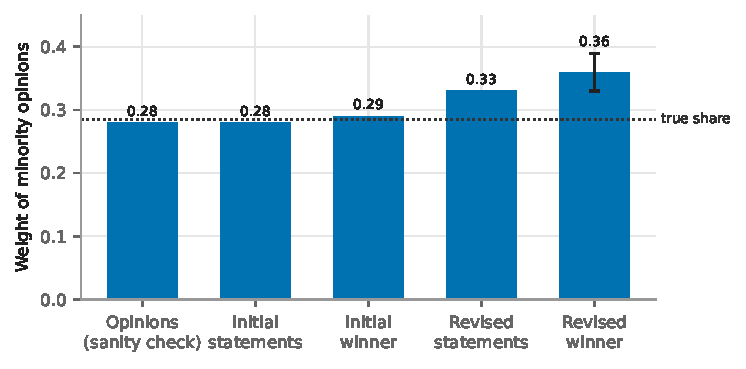
\includegraphics[width=0.95\linewidth]{figures/fig_paper.pdf}
\caption{\fillin{The paper's own result, redrawn from the data labels of SM Figure S60
(``Position Embedding'' panel), which SM 5.2.2 identifies as the expanded version of main-text
Figure 4C. Dotted line: the true proportion of minority opinions (\paperShare). Error bar on the
revised winner: $\pm\paperRevWinSE$, one standard error of the estimated regression coefficient,
as printed in the paper. $n=\paperNRounds$ rounds.}}
\label{fig:paper}
\end{figure}

\section*{What is a minority (or majority) group?}
\codebox{\codeMinority}

In the papers' experiments, groups of between \fillin{\groupMin--\groupMax} people took part in
the deliberative process mediated by the HM. Before writing their free-text opinion, they indicated
their level of agreement with a political proposition using a Likert scale of 1--7. It was thus
possible to provide a neutral (4) opinion. A group was defined as having a minority group if there
was an unequal amount of agreeing (5--7) and disagreeing (1--3) opinions. Groups without a minority
group were excluded from this analysis.

\fillin{\textbf{Reproduction parameters.} The primary sample is the pre-registered groups of
cohorts 1--3: \groupNRounds{} rounds, of which \oursNRoundsLarge{} contain a minority under this
rule, giving a true minority share of \oursShareLarge{}.}\footnote{\fillin{The paper reports
\paperShare{}. The gap is almost entirely the treatment of neutral raters. SM 5.4.1 counts a
neutral (4) rating as non-minority: ``we may define the `minority' side of the Likert scale as the
side that contains the smaller number of opinions, and define all other opinions as `non-minority'
opinions---which include `majority' opinions [\ldots] as well as `neutral' opinions (i.e.\ with a
Likert rating of 4), if any.'' Applied literally, with rounds that have equal numbers on each side
excluded, that rule gives \oursShareLarge{} on these rounds. Two other readings land on the
paper's figure: dropping neutral raters from their groups before the sides are counted gives
\shareRuleNeutralDropped{} (\shareRuleNeutralDroppedNRounds{} rounds), and keeping the tied rounds
with a fixed side taken as the minority gives \shareRuleTiesKept{} (\shareRuleTiesKeptNRounds{}
rounds). The treatment of neutral raters is carried through the
\hyperref[sec:sensitivity]{sensitivity analysis} below.}}

\section*{How does the HM paper measure how well-represented minority opinions are?}

This part of the analysis has two components. First, each participant's free-text opinion and the
statements produced by the HM (including intermediate statements produced in its iterative process)
are given a scalar score to measure to what extent they agree or disagree with the political
proposition. I refer to this score as the ``position component score''.\footnote{\fillin{The name
follows SM 5.1.1, where the position component of a text embedding is its value along the position
axis. It is best understood as a way of measuring the level of agreement with the proposition,
similar to a political valence score: a single number that places a text between the negating and
the affirming position on the question.}}

The position component scores of original human opinions and LLM-generated statements are then
used to measure how similar the average position component scores among a minority group are, to
the position component score of the LLM-generated statement.

I now detail my reproduction of each of these steps.

\section*{Measuring the position component score}
\codebox{\codeAgreement}

To measure the position component score of a human-authored opinion or a LLM-generated statement,
it is first mapped into a 768-dimension embedding, and then projected onto the vector going between
two points.\footnote{\fillin{SM 5.1.2 gives the method for constructing the two endpoints --- a
generic prefix (``Yes, I agree.'' or ``No, I disagree.'') concatenated with the question's own
affirming or negating position statement --- and one illustrative example, but not the exact
phrases used for each question. Here each endpoint is the prefix followed by the position statement
released with the data; the axis is the unit vector from the negating to the affirming endpoint (SM
eq.~3) and the score is the projection onto it (SM eq.~5).}}

The main detail missing from the SM is what exact embedding model was used for this process. While
the SM describes Sentence-T5, there are various sizes of this model that could be used.

\subsection*{Validating the position component score}
\codebox{\codeAgreementValidation}

The original authors validate their position component score method by using the original human
responses, comparing the human's self-reported Likert scores against the estimated position
component scores derived from the method above. In the original paper, they report an $R^2$ of
\paperMarginalRsq{}.\footnote{\fillin{The paper does not say exactly how this $R^2$ is computed.
\hyperref[app:rsq]{Appendix~A} sets out the candidate definitions, how I settled on one, the
regression that produces it, and its value under each embedding model.}} In our reproduction, the
$R^2$ of each embedding model is shown in Table~\fillin{\ref{tab:rsq}}
\fillin{(\hyperref[app:rsq]{Appendix~A})}.

Based on these results, we choose model \fillin{sentence-t5-large} as the most-likely model used in
the original analysis. \fillin{Its marginal $r^2$ of \oursMarginalRsqLarge{} is within
\oursMarginalRsqGapLarge{} of the paper's \paperMarginalRsq{}, and its Pearson $r$ of
\oursPearsonRLarge{} against the paper's \paperFigAr{} says the same thing: the position axis this
report is built on is about as good as the one the paper used. The other size that could be run
here, sentence-t5-base, enters the \hyperref[sec:sensitivity]{sensitivity analysis} as the
alternative model.}

\section*{Measuring representativeness}
\codebox{\codeRepresentation}

Given a set of human-authored opinions $\{x_i \mid i \in 1,\dots,n\}$, a partition of opinions into
minority $M$ \& non-minority $N$ sets, position component scores $\{a_i \mid i \in 1,\dots,n\}$,
the ``representation'' of an opinion $x_i$ is given by $\lambda_i$ in
%
\begin{equation*}
\text{set } \lambda_i \text{ to minimise } \Big(a_0 - \sum_i \lambda_i a_i\Big)^2
\qquad\text{such that}\qquad \sum_i \lambda_i = 1 \ \ \&\ \ \lambda_i \geq 0 .
\end{equation*}
%
To calculate the representation of $M$ \& $N$, simply calculate the average representation of their
elements: $\lambda_M := \frac{1}{|M|}\sum_{x_i \in M} \lambda_i$.

\subsection*{The implementation check}
\codebox{\codeSanity}

To test that the implementation of this procedure works as expected, the original authors ran a
check where \fix{each human opinion in turn is treated as the target and regressed on convex
combinations of that same set of opinions. Averaged over the set, the recovered minority weight
should come back as simply the proportion of opinions in the
minority.}\footnote{Corrected. The draft read: ``the output statement was simply one of the $m$
human opinion inputs, and repeated this $m$ times (once for each input). [this may be incorrect]
After averaging across these runs, the average representation $\bar\lambda_i$ of an input $x_i$
should be $\frac{1}{m}$.'' The draft's own flag was right. The paper's Materials and Methods
describe it as: ``As a sanity check, we similarly regress individual opinions on convex
combinations of those same opinions, which we verify to simply yield the proportion of opinions in
the minority.'' The target of the check is the \emph{minority share}, not $1/m$ per input.} We
replicate this implementation check. \fillin{It passes: the recovered weight is
\oursOpinionsLarge{} against a true share of \oursShareLarge{}; the paper reports
\paperOpinions{} against its true share of \paperShare{}. This is the leftmost bar of
Figure~\ref{fig:contrast}.}

\section*{Results}
\phantomsection\label{sec:results}
\codebox{\codeResults}

We fail to replicate the results from the original paper. Figure~\fillin{\ref{fig:contrast}}
displays an adjusted version of Figure~\fillin{\ref{fig:paper}} above, where we contrast the
original paper's results against our own.\footnote{\fillin{Error bars in both figures are $\pm 1$
standard error of the estimated regression coefficients, which is how SM Figure S60 defines them.
The SM does not say how that standard error is obtained for a constrained regression. Here the
constrained fit is treated as an ordinary least-squares fit on its active set (the coefficients
above zero) with the sum-to-one constraint eliminated; the standard error of the summed minority
coefficients is read from the resulting covariance matrix, and the level-specific standard errors
are combined with the same round-count weights as the estimate itself (SM eq.~19). As a check on
that construction, a cluster bootstrap over rounds gives a standard error of
\oursRevWinBootSELarge{} for the revised winner against the analytic \oursRevWinSELarge{}.}}

\begin{figure}[h]
\centering
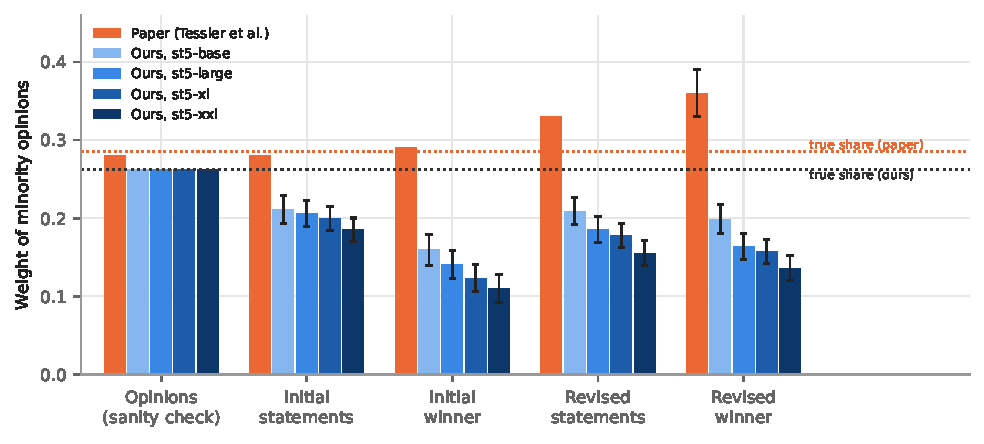
\includegraphics[width=\linewidth]{figures/fig_contrast.pdf}
\caption{\fillin{Minority weight at each phase: the paper against this reproduction under
sentence-t5-large. Error bars are $\pm 1$ standard error of the estimated regression coefficients,
as in SM Figure S60. The two dotted lines are the true minority share in each case (\paperShare{}
for the paper, \oursShareLarge{} here; the difference is the treatment of neutral raters).
$n=\oursNRoundsLarge$ rounds with a minority, from \oursNRoundsTotalLarge{} pre-registered rounds
in cohorts 1--3.}}
\label{fig:contrast}
\end{figure}

\fillin{Three observations: 1) The sanity check reproduces exactly --- the leftmost bars sit on
their respective true shares --- so the regression machinery is doing what the paper says it does.
2) Every statement phase, by contrast, sits below the true share rather than at or above it: the
revised winner carries \oursRevWinLarge{} $\pm$ \oursRevWinSELarge{} against the paper's
\paperRevWin{}. 3) The shape differs: in the paper the four phases rise monotonically, whereas here
the winner-selection step \emph{drops} minority weight at both rounds (initial candidates
\oursInitCandLarge{} $\rightarrow$ initial winner \oursInitWinLarge{}), and the revision step
partially restores it (\oursRevWinLarge{}). The paper's rise from initial winner to revised winner
is therefore present ($+\diffWinToWinLarge$, 95\% CI $[\diffWinToWinCIloLarge,
\diffWinToWinCIhiLarge]$, $p=\diffWinToWinPLarge$), but it starts from a lower base and does not
carry the final statement above proportionality; measured from the initial candidates instead, the
change over the whole process is $\diffInitToFinalLarge$ (95\% CI $[\diffInitToFinalCIloLarge,
\diffInitToFinalCIhiLarge]$).}

\subsection*{Validation checks}
\codebox{\codeValidationExtra}

\fillin{Everything above is only interesting if the pipeline is sound, so the checks that bear on
that are collected in Table~\ref{tab:validation}. Three of the four independent checks land on the
paper's values, which is the basis for reporting the disagreement rather than assuming a bug. The
one that does not --- the share of statements falling inside the range of their group's opinions
--- is lower here than in the paper, and is the clearest remaining candidate for an unmodelled
difference.}

\begin{table}[h]
\centering
\small
\caption{\fillin{Checks on the reproduction, independent of the minority-weight result.}}
\label{tab:validation}
\begin{tabular}{p{7.4cm}cc}
\toprule
\fillin{check} & \fillin{paper} & \fillin{ours (sentence-t5-large)} \\
\midrule
\fillin{Sanity check: opinions regressed on themselves recover the minority share} & \fillin{\paperOpinions{} vs \paperShare{}} & \fillin{\oursOpinionsLarge{} vs \oursShareLarge{}} \\
\fillin{Position axis quality: marginal $r^2$ of Likert on position component score} & \fillin{\paperMarginalRsq} & \fillin{\oursMarginalRsqLarge} \\
\fillin{Fig.\ 4A: correlation of position component score with Likert rating} & \fillin{\paperFigAr} & \fillin{\oursFigArLarge} \\
\fillin{Fig.\ 4B: statements falling within the range of their group's opinions} & \fillin{\paperFigBwithin} & \fillin{\oursFigBwithinLarge} \\
\bottomrule
\end{tabular}
\end{table}

\section*{Sensitivity analysis}
\phantomsection\label{sec:sensitivity}
\codebox{\codeSensitivity}

As noted above, there are several aspects of the analysis plan which are not specified in the SM.
These are:

\begin{table}[h]
\centering
\small
\caption{\fillin{Underspecified choices, the options considered, and the option taken in the
primary specification above.}}
\label{tab:ambiguity}
\begin{tabular}{p{4.1cm}p{6.2cm}p{4.4cm}}
\toprule
\fillin{ambiguity} & \fillin{possible options} & \fillin{option chosen above} \\
\midrule
\fillin{ST5 model size} & \fillin{base, large, xlarge, xxl} & \fillin{large (\hyperref[app:rsq]{Appendix~A})} \\
\fillin{Neutral (Likert 4) raters} & \fillin{count as non-minority; drop the rater; drop the whole group} & \fillin{count as non-minority (SM 5.4.1)} \\
\fillin{Basis for splitting minority / non-minority} & \fillin{Likert rating; sign of the position component score (SM Fig.\ S62)} & \fillin{Likert rating (SM Fig.\ S60)} \\
\fillin{Column order: how a round's opinions are assigned to the regressors} & \fillin{order in the released data; sorted by position component score; random} & \fillin{data order} \\
\bottomrule
\end{tabular}
\end{table}

\fillin{The last row needs a word of explanation. The regression at each level of division fits one
coefficient per column of the design matrix, and each row of that matrix is one round's opinion
scores, so a column pools ``the $j$-th opinion'' across rounds. SM eq.~13 indexes a round's
opinions by $j$ without saying how $j$ is assigned. Here the minority opinions always occupy the
first columns, and the three options above fix the order within the minority block and within the
non-minority block. The minority weight sums the minority columns, which removes the dependence
on order within the minority block when the minority has one member, but the order of the
non-minority columns still changes the fit.}

I reran the analysis with every combination of these decisions
(\fillin{\sensNRuns{}} runs).\footnote{\fillin{Two model sizes $\times$ three neutral-rater
treatments $\times$ three column orders when the split is by Likert rating, plus two model sizes
$\times$ three column orders when the split is by the sign of the score, where there are no neutral
raters: \sensNRuns{} runs, \sensNRunsPerModel{} per model. The xlarge and xxl sizes could not be
run here (\hyperref[app:rsq]{Appendix~A}).}} Across the runs, I calculated the following metrics:

\begin{itemize}[leftmargin=1.4em,itemsep=0.25em]
  \item Proportion of runs where minority representation increases from initial to final:
        \fillin{\sensPropInitToFinal{}}
  \item Proportion of runs where minority representation is larger in final than the prevalence
        among population (\fix{\oursShareLarge}):\footnote{Corrected. The draft gave 0.291. That is
        the true share under one variant --- neutral raters dropped --- not under the primary
        specification, where it is \oursShareLarge{}. Each run is compared against its own true
        share rather than a single fixed number, since the minority rule changes the share as well
        as the weight.}
        \fillin{\sensPropAboveShare{}. The largest revised-winner weight in the sweep is
        \sensMaxRevWin{}, against a mean true share of \sensTrueShareMean{}.}
  \item Average representation at each of the 4 stages, with the range across runs:
        \fillin{shown in Figure~\ref{fig:sensitivity}.}
\end{itemize}

\begin{figure}[t]
\centering
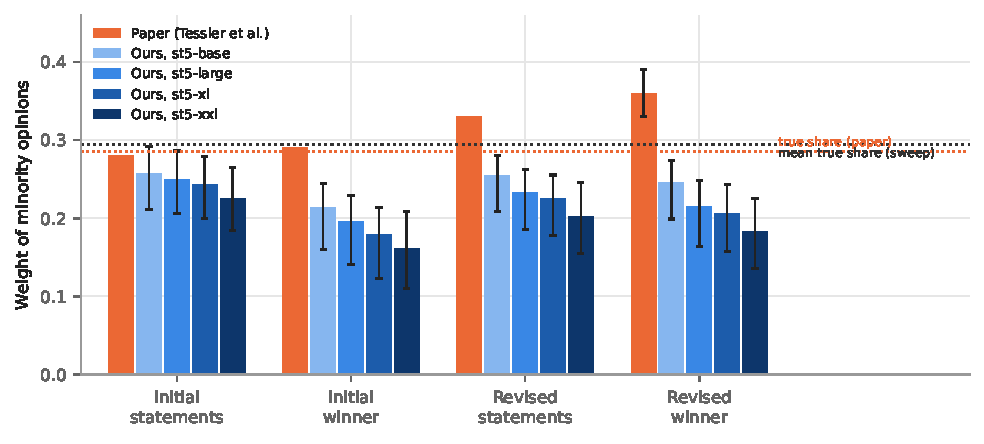
\includegraphics[width=0.92\linewidth]{figures/fig_sensitivity.pdf}
\caption{\fillin{Mean minority weight at each phase across the \sensNRunsPerModel{} specifications
run under each embedding model; whiskers span the full range (minimum to maximum) of those
specifications. Dotted line: the mean true minority share across all \sensNRuns{} runs
(\sensTrueShareMean{}). No specification places the revised winner above its own true share.}}
\label{fig:sensitivity}
\end{figure}

\section*{Discussion}

If the above reproduction of the analysis pipeline is correct, then it would appear that the HM
actually suppresses minority opinions, if we follow the original paper's interpretation of the
above measurement method.

Notably, we are able to reproduce several parameter estimates from the paper, including the
validation of the embedding-based position component score and the implementation check of the
regression method. We fail to replicate the substantive findings for this part of the paper,
however.

This finding actually aligns somewhat with the finding that people's beliefs shifted towards the
majority position (although there are many possible explanations for this finding).

\clearpage
\section*{Appendix A: the paper's $R^2$ statistic}
\phantomsection\label{app:rsq}
\codebox{\codeAgreementValidation}

\fillin{\textbf{What the paper says.} The main text reports: ``A random-effects estimator of the
regression coefficient for Likert ratings on position embeddings yields a marginal r-squared value
of \paperMarginalRsq{} (SM 5.1.3).'' SM 5.1.3 adds that a model taking the top ten residual
embedding components as additional inputs has marginal and conditional $r^2$ of \paperMarginalRsq{}
and \paperConditionalRsq{}, ``similar to the model containing only the position component''. That
leaves three things unspecified: which $R^2$ is meant --- the marginal $R^2$ of a mixed model, or
the plain Pearson $r^2$ of the scatter in Figure 4A, whose $r=\paperFigAr{}$ squares to
\paperFigArSq{}; what the random effect is grouped by (question, round or participant); and whether
only the intercept or also the slope varies by group.}

\fillin{\textbf{How I settled on a definition.} ``Marginal'' and ``conditional'' $r^2$ are the
standard names for the Nakagawa--Schielzeth decomposition of variance explained in a mixed model,
and the main text names a random-effects estimator, so I take the statistic to be the marginal
$R^2$ of a random-intercept model. I group by round, the unit at which a group forms and a question
is answered, and let only the intercept vary, since a random slope would add a further unstated
choice. Because the paper's Pearson $r^2$ and its marginal $R^2$ coincide at \paperMarginalRsq{},
the paper's own number cannot separate the two definitions, so Table~\ref{tab:rsq} reports both.
Under either definition the ranking of the embedding models, and with it the choice of
sentence-t5-large, is the same.}

\fillin{\textbf{The regression.} For participant $j$ in round $i$, with Likert rating $y_{ij}$ and
position component score $s_{ij}$,
\begin{equation*}
y_{ij} = \alpha + \beta\, s_{ij} + u_i + \varepsilon_{ij}, \qquad
u_i \sim \mathcal{N}(0, \sigma_u^2), \quad \varepsilon_{ij} \sim \mathcal{N}(0, \sigma_\varepsilon^2),
\end{equation*}
fitted by restricted maximum likelihood on the \oursMixedNLarge{} opinions of the
\oursMixedNRoundsLarge{} pre-registered rounds of cohorts 1--3. Writing $\sigma_f^2$ for the
variance of the fixed-effect predictions $\hat\beta s_{ij}$,
\begin{equation*}
R^2_{\text{marginal}} = \frac{\sigma_f^2}{\sigma_f^2 + \sigma_u^2 + \sigma_\varepsilon^2},
\qquad
R^2_{\text{conditional}} = \frac{\sigma_f^2 + \sigma_u^2}{\sigma_f^2 + \sigma_u^2 + \sigma_\varepsilon^2}.
\end{equation*}
Under sentence-t5-large the fitted slope is $\hat\beta = \oursMixedBetaLarge{}$ (SE
\oursMixedBetaSELarge{}); under sentence-t5-base it is \oursMixedBetaBase{} (SE
\oursMixedBetaSEBase{}).}

\begin{table}[h]
\centering
\small
\caption{\fillin{Fit of the position component score to the Likert rating, by embedding model:
marginal and conditional $r^2$ of the random-intercept model above, and the Pearson correlation
of the raw scatter (the main-text Figure 4A quantity) with its square.}}
\label{tab:rsq}
\begin{tabular}{lcccc}
\toprule
 & marginal $r^2$ & conditional $r^2$ & Pearson $r$ & Pearson $r^2$ \\
\midrule
\fillin{sentence-t5-base}   & \fillin{\oursMarginalRsqBase}  & \fillin{\oursConditionalRsqBase}  & \fillin{\oursPearsonRBase}  & \fillin{\oursPearsonRsqBase} \\
\fillin{sentence-t5-large}  & \fillin{\oursMarginalRsqLarge} & \fillin{\oursConditionalRsqLarge} & \fillin{\oursPearsonRLarge} & \fillin{\oursPearsonRsqLarge} \\
\fillin{sentence-t5-xlarge} & \multicolumn{4}{c}{\fillin{not evaluated --- see note}} \\
\midrule
\fillin{paper}              & \fillin{\paperMarginalRsq} & \fillin{\paperConditionalRsq} & \fillin{\paperFigAr} & \fillin{\paperFigArSq} \\
\bottomrule
\end{tabular}
\end{table}

\fillin{The xlarge row is empty for a hardware reason rather than a scientific one: sentence-t5-xl
is a 3B-parameter model and this machine has no GPU and 7~GB of RAM, so it could not be embedded
here. The two sizes that could be run bracket the question well enough to answer it --- base falls
well short of the paper's \paperMarginalRsq{} and large lands essentially on it --- and the
direction of the remaining risk is worth stating plainly: if the authors used a larger ST5 than
large, the axis would be slightly \emph{better} than mine, and a better axis moves the minority
weight further from the paper's value, not closer (\hyperref[sec:sensitivity]{Sensitivity
analysis}).}

\end{document}
